\documentclass[11pt,a4paper]{article}
\usepackage[utf8]{inputenc}
\usepackage[margin=1in]{geometry}
\usepackage{titlesec}
\usepackage{enumitem}
\usepackage{xcolor}
\usepackage{tcolorbox}
\usepackage{fancyhdr}
\usepackage{hyperref}
\usepackage{graphicx}
\setlength{\headheight}{14pt}

% Colors
\definecolor{teal}{HTML}{4A9E8F}
\definecolor{orange}{HTML}{E8945A}
\definecolor{lime}{HTML}{B8CC4B}

% Section formatting
\titleformat{\section}{\Large\bfseries\color{teal}}{Slide \thesection:}{0.5em}{}
\titlespacing{\section}{0pt}{20pt}{10pt}

% Header/Footer
\pagestyle{fancy}
\fancyhf{}
\fancyhead[L]{\textcolor{teal}{\textbf{sTiles Presentation Script}}}
\fancyhead[R]{\textcolor{gray}{SIAM PP26}}
\fancyfoot[C]{\thepage}
\renewcommand{\headrulewidth}{0.4pt}

% Speech box
\newtcolorbox{speech}{
    colback=gray!5,
    colframe=teal,
    fonttitle=\bfseries,
    title=Speaker Notes,
    boxrule=0.5pt,
    arc=2pt
}

\begin{document}

\begin{center}
{\Huge\bfseries\color{teal} Speaker Script}\\[0.5em]
{\Large sTiles: Accelerated Computational Framework}\\[0.3em]
{\large for Sparse Factorizations of Structured Matrices}\\[1em]
{\normalsize SIAM Conference on Parallel Processing (PP26) --- March 2026}
\end{center}

\vspace{1em}
\hrule
\vspace{1em}

\noindent\textbf{Total Presentation Time:} 25--30 minutes\\
\textbf{Style:} Professional, clear, technically precise\\
\textbf{Coverage:} Two papers (ISC25 + ISC26) plus additional updates

\vspace{2em}

%==============================================================================
\section{Title Slide}
\begin{center}
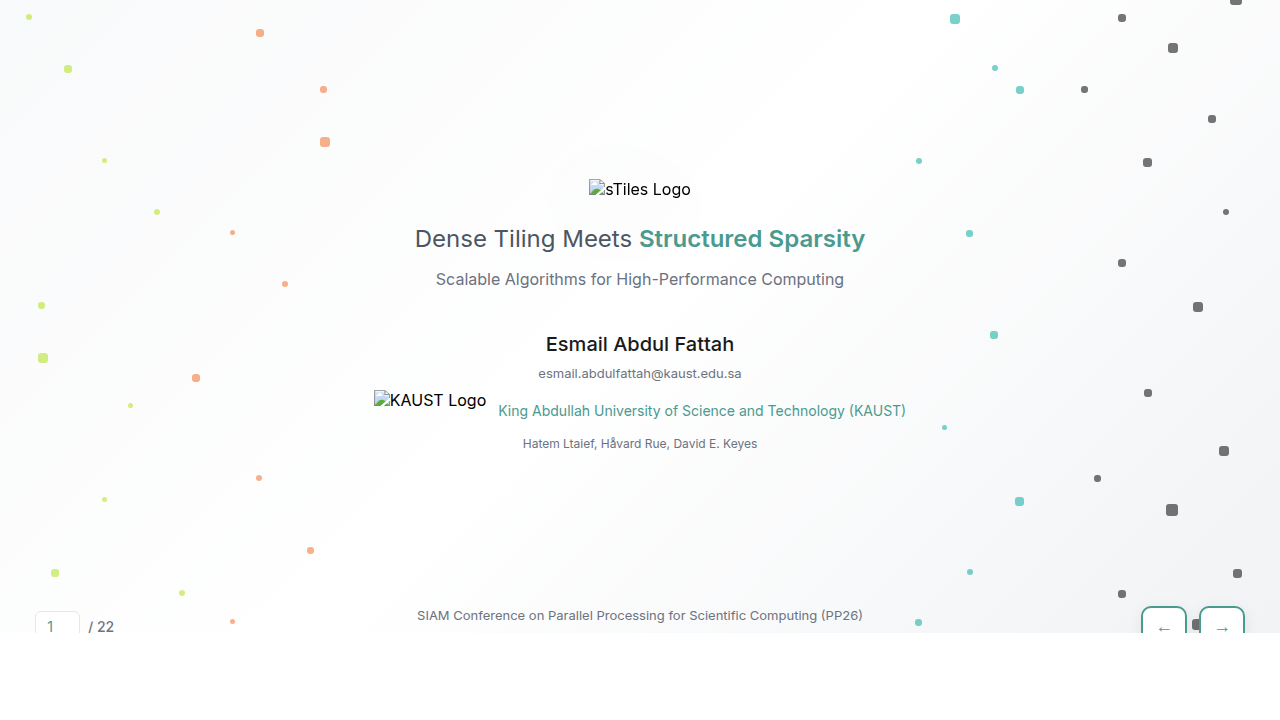
\includegraphics[width=\textwidth]{slide_screenshots/slide_01.png}
\end{center}
%==============================================================================

\begin{speech}
Good morning/afternoon everyone. Thank you for attending this session.

Today I'll present sTiles, our GPU-accelerated computational framework for sparse factorizations of structured matrices. This work represents two papers --- one on Cholesky factorization published at ISC25, and one on selected inversion targeting ISC26 --- plus additional optimizations we've developed since.

The practical motivation is enabling faster Bayesian inference at scale, where these factorizations are the computational bottleneck.
\end{speech}

\vspace{1em}

%==============================================================================
\section{Why This Matters}
\begin{center}
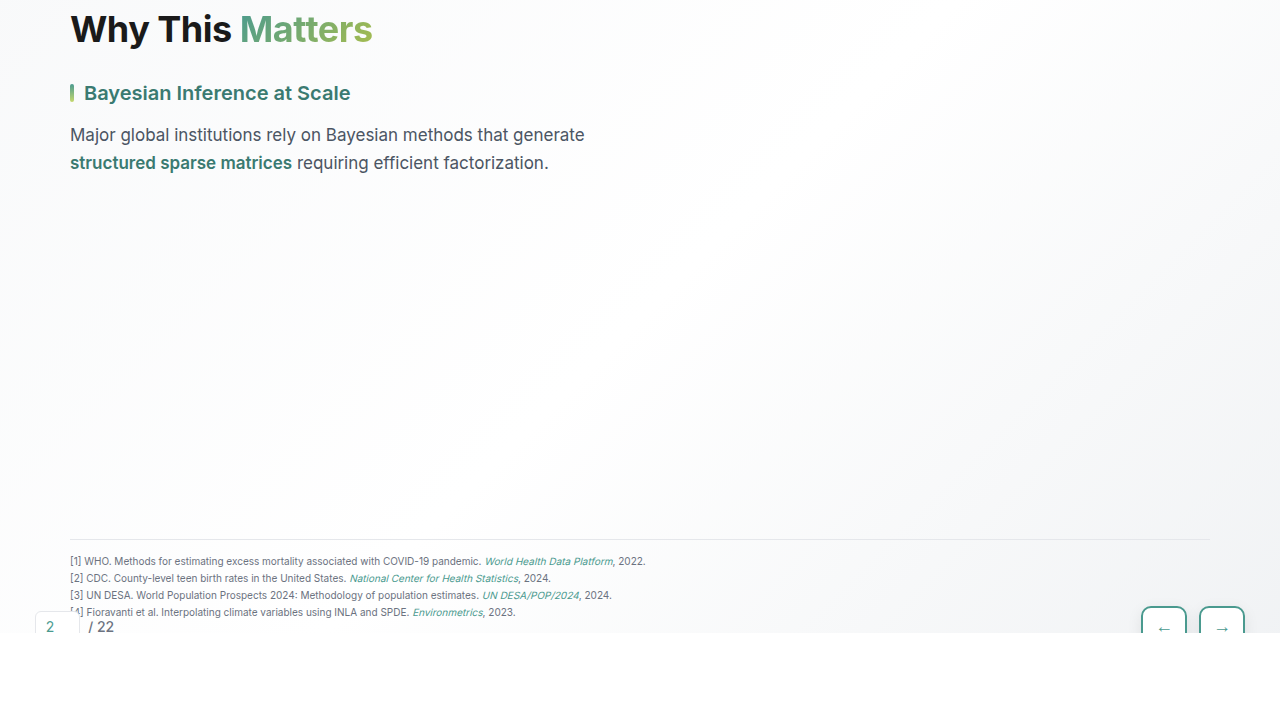
\includegraphics[width=\textwidth]{slide_screenshots/slide_02.png}
\end{center}
%==============================================================================

\begin{speech}
Let me start with why this work matters beyond pure linear algebra.

Major global institutions --- the World Health Organization, the CDC, the United Nations --- all rely on Bayesian statistical methods for critical analyses. WHO used these techniques to estimate excess COVID-19 mortality. The CDC uses them for epidemiological studies. The UN uses them for World Population Prospects.

All these applications use a methodology called INLA --- Integrated Nested Laplace Approximations --- which requires \textbf{hundreds} of Cholesky factorizations and selected inversions per inference run.

The matrices involved are \textbf{structured sparse} matrices, typically arrowhead patterns from Kronecker products of spatial and temporal components. As data resolution increases --- more sensors, finer time steps, larger geographic coverage --- these matrices grow larger and denser.

This is where sTiles comes in: we need efficient factorization that exploits this structure.
\end{speech}

\vspace{1em}

%==============================================================================
\section{INLA: Global Impact}
\begin{center}
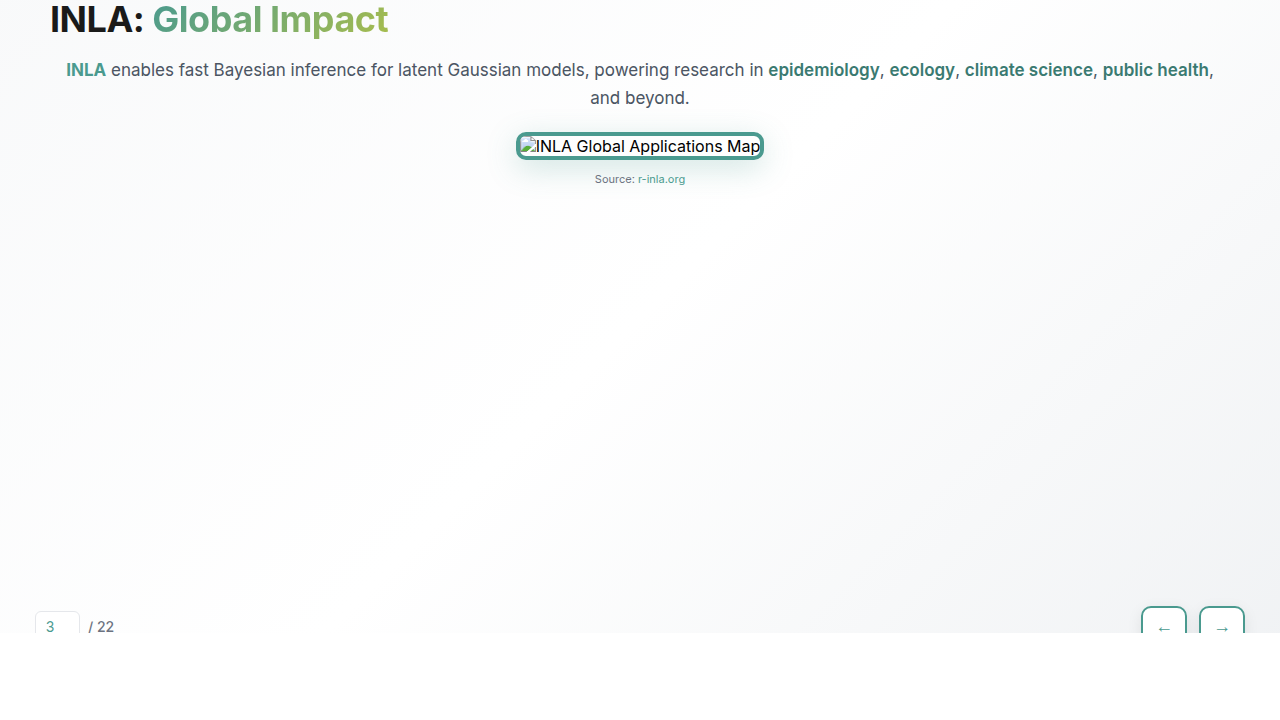
\includegraphics[width=\textwidth]{slide_screenshots/slide_03.png}
\end{center}
%==============================================================================

\begin{speech}
This map shows the global reach of INLA-based research.

INLA enables fast approximate Bayesian inference for latent Gaussian models. It's become the standard tool in spatial statistics, with applications spanning epidemiology, ecology, climate science, and public health.

The R-INLA package has been used in thousands of published papers across these domains.

Every dot on this map represents research that depends on efficient sparse matrix computations. That's the scale of impact we're targeting with sTiles.
\end{speech}

\vspace{1em}

%==============================================================================
\section{The Computational Challenge}
\begin{center}
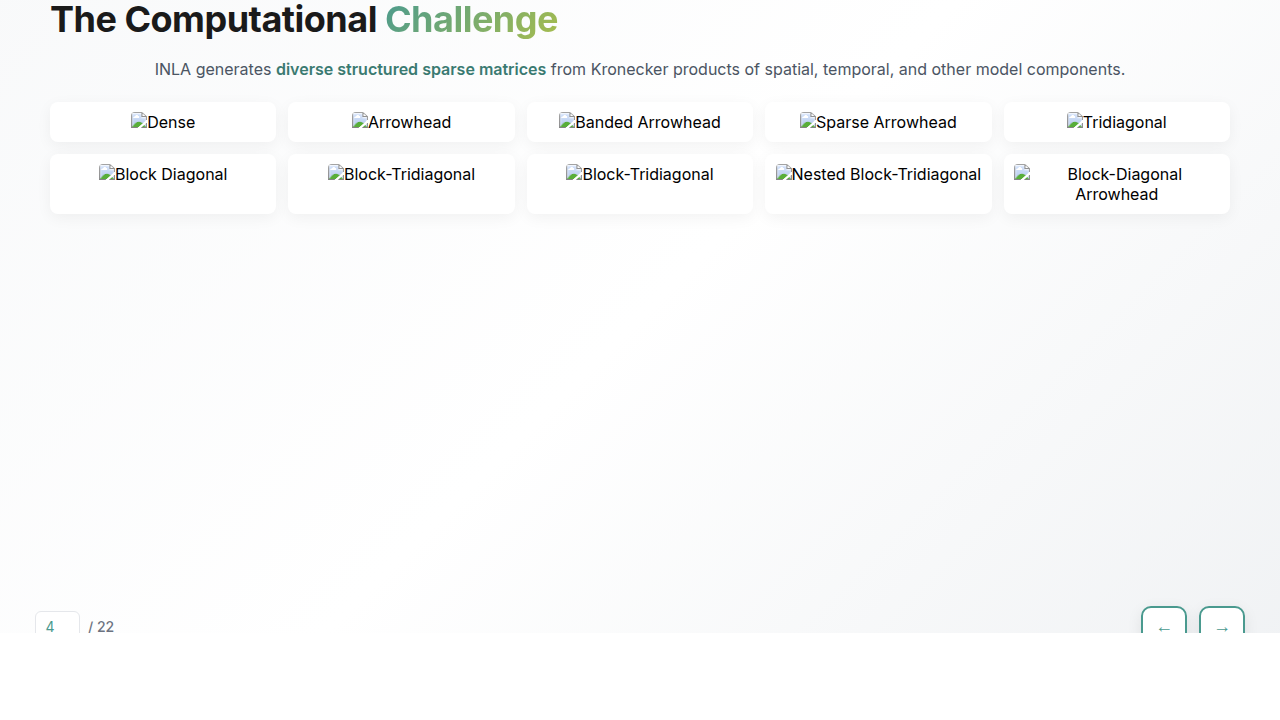
\includegraphics[width=\textwidth]{slide_screenshots/slide_04.png}
\end{center}
%==============================================================================

\begin{speech}
INLA generates diverse structured sparse matrices from Kronecker products of model components --- spatial fields, temporal dynamics, fixed effects.

Here you can see ten different sparsity patterns we encounter: dense, arrowhead, banded arrowhead, sparse arrowhead, tridiagonal, block diagonal, block tridiagonal with arrowhead, and various nested block structures.

The challenge is that \textbf{neither traditional sparse nor dense solvers are optimal} for these matrices.

\textit{[Advance to show solver comparison]}

Sparse solvers like CHOLMOD or PARDISO have low arithmetic intensity. They're designed for scattered sparsity, not dense clusters. They suffer from poor cache utilization and irregular memory access.

Dense solvers like PLASMA have $O(n^3)$ complexity. They ignore the sparsity pattern entirely, wasting memory on zeros.

\textit{[Advance to show key message]}

Neither approach is optimal! We need the efficiency of sparse methods combined with the performance of dense BLAS kernels. That's exactly what sTiles provides.
\end{speech}

\vspace{1em}

%==============================================================================
\section{The sTiles Approach}
\begin{center}
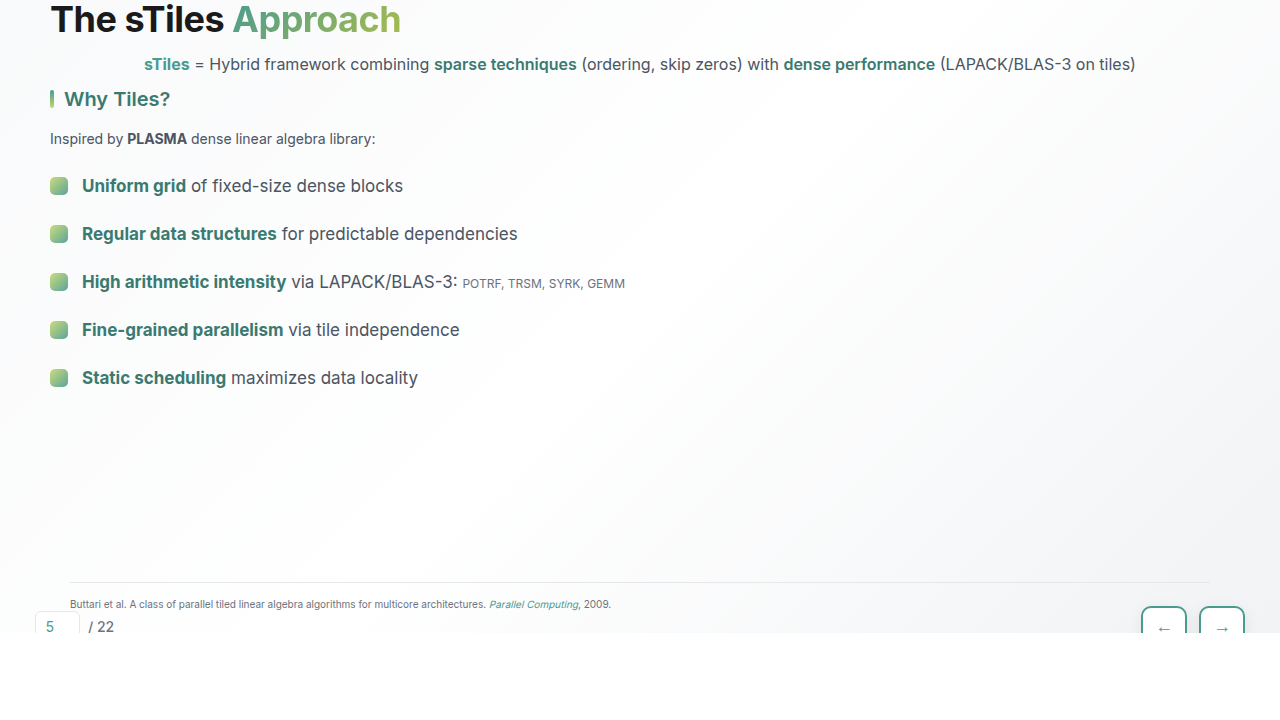
\includegraphics[width=\textwidth]{slide_screenshots/slide_05.png}
\end{center}
%==============================================================================

\begin{speech}
sTiles is a hybrid framework combining sparse techniques with dense performance.

The key insight comes from PLASMA, the dense linear algebra library: partition the matrix into \textbf{uniform fixed-size tiles} and operate on them using highly optimized LAPACK and BLAS-3 kernels --- POTRF, TRSM, SYRK, GEMM.

This gives us regular data structures with predictable dependencies, high arithmetic intensity from BLAS-3 operations, fine-grained parallelism through tile independence, and static scheduling that maximizes data locality.

\textit{[Advance to show sparse techniques]}

But we don't treat everything as dense. We preserve sparsity through preprocessing: permutation using RCM, AMD, or Nested Dissection to minimize fill-in; symbolic factorization to identify which tiles will be nonzero; and most importantly, we \textbf{skip zero tiles entirely} during computation.

\textit{[Advance to show tile visualization]}

Here's the transformation: sparse points become dense tiles. For this banded arrowhead example, we only compute 44 of 100 possible tiles. The gray tiles are never allocated or touched.

This is the essence of sTiles: dense operations where it matters, nothing where it doesn't.
\end{speech}

\vspace{1em}

%==============================================================================
\section{The Fill-in Challenge}
\begin{center}
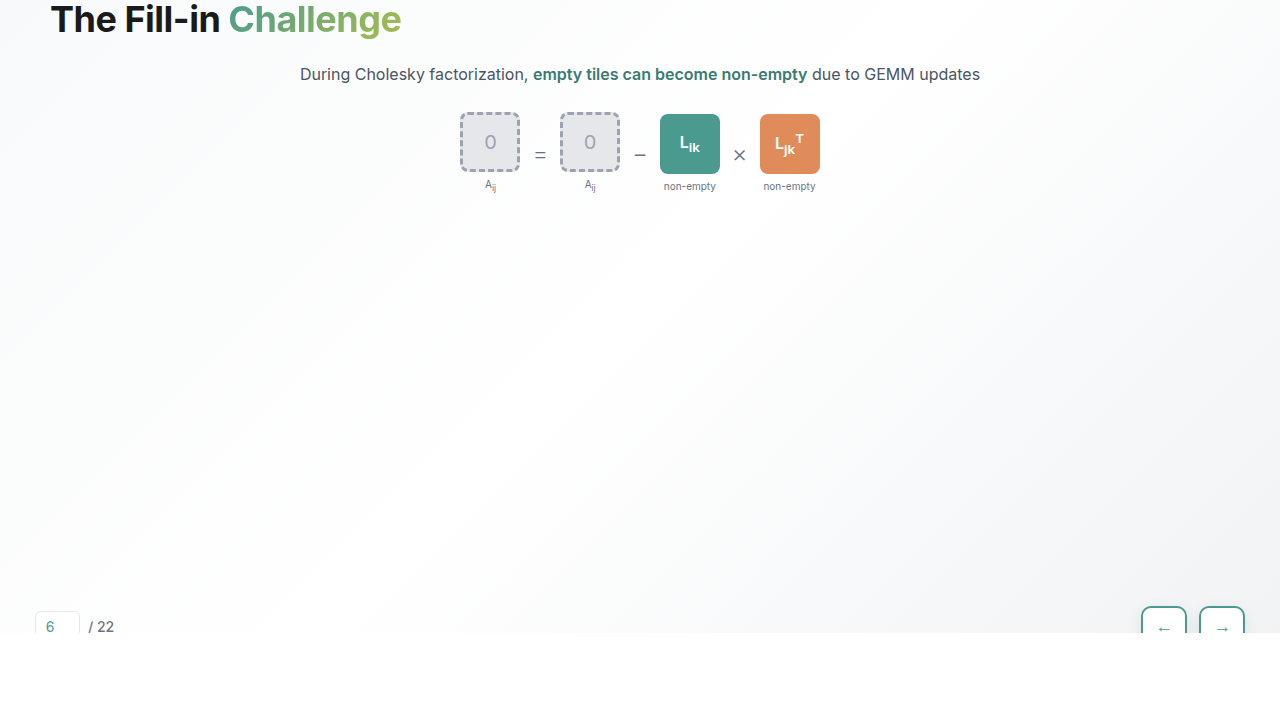
\includegraphics[width=\textwidth]{slide_screenshots/slide_06.png}
\end{center}
%==============================================================================

\begin{speech}
Before we can skip zero tiles, we need to know which tiles will remain zero. This is the fill-in challenge.

During Cholesky factorization, a GEMM update can create fill-in: a tile that starts empty can become non-empty.

Look at this equation: $A_{ij}$ starts as zero. But if both $L_{ik}$ and $L_{jk}$ are non-empty, then the product $L_{ik} \times L_{jk}^T$ is non-zero, and $A_{ij}$ gets filled in.

\textit{[Advance to show fill-in result]}

This tile is now allocated and must be computed. We can't skip it.

The symbolic factorization phase determines exactly which tiles will have fill-in. Once we know that, we allocate only those tiles and compute only those operations.

For arrowhead matrices with natural ordering, fill-in is \textbf{predictable and structured}. The arrowhead shape is preserved in the Cholesky factor, which is why these matrices are particularly amenable to our approach.
\end{speech}

\vspace{1em}

%==============================================================================
\section{The Memory Trade-off}
\begin{center}
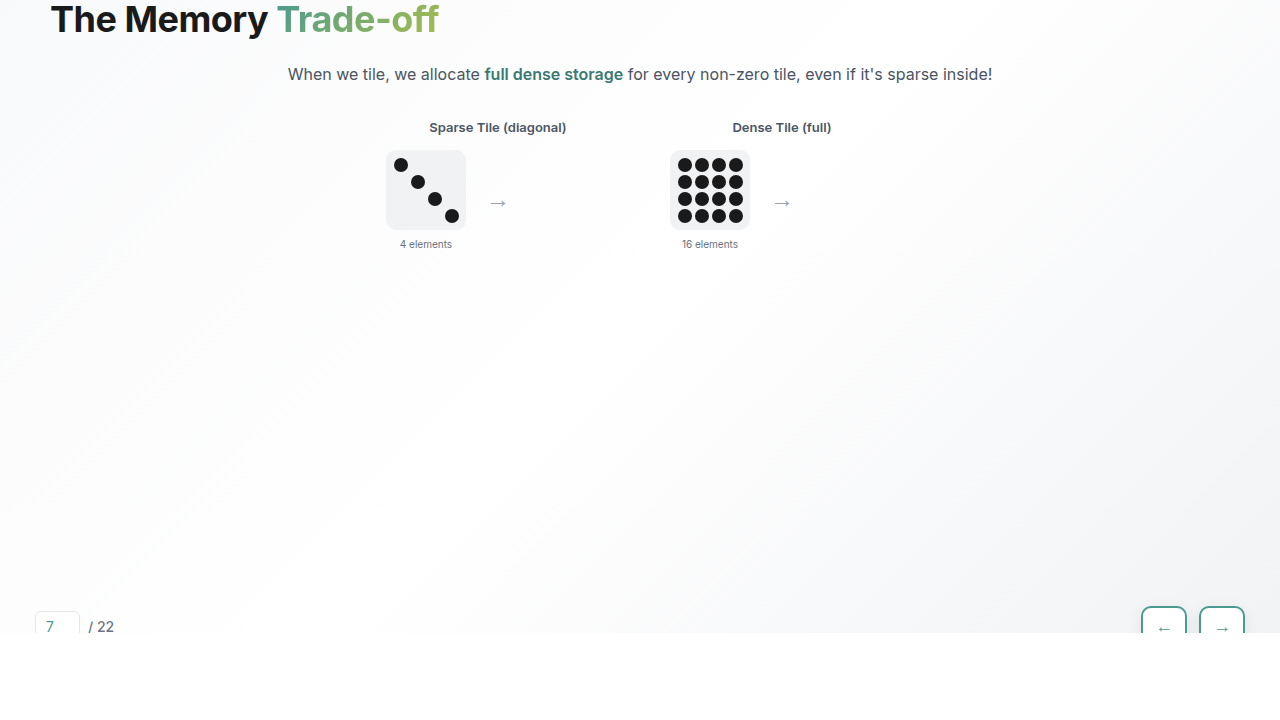
\includegraphics[width=\textwidth]{slide_screenshots/slide_07.png}
\end{center}
%==============================================================================

\begin{speech}
There's an important trade-off with tile-based approaches: when we tile, we allocate \textbf{full dense storage} for every non-zero tile, even if it's sparse inside.

Consider a sparse diagonal tile with only 4 elements on the diagonal. We still allocate storage for all 16 elements in that tile.

\textit{[Advance to show allocation]}

The sparse tile uses the same memory as a fully dense tile!

Is this worth it? Yes, when the tiles are dense enough. The benefit is that we can use highly optimized dense BLAS kernels without any sparse indexing overhead. For diagonal tiles that are truly sparse, we can use customized kernels or smaller tile sizes.

\textit{[Advance to show tile sizes]}

The optimal tile size depends on the architecture. For CPUs, we use approximately 120 to fit in L2/L3 cache. For GPUs, we use approximately 600 to maximize occupancy and kernel efficiency.
\end{speech}

\vspace{1em}

%==============================================================================
\section{Ordering Strategies}
\begin{center}
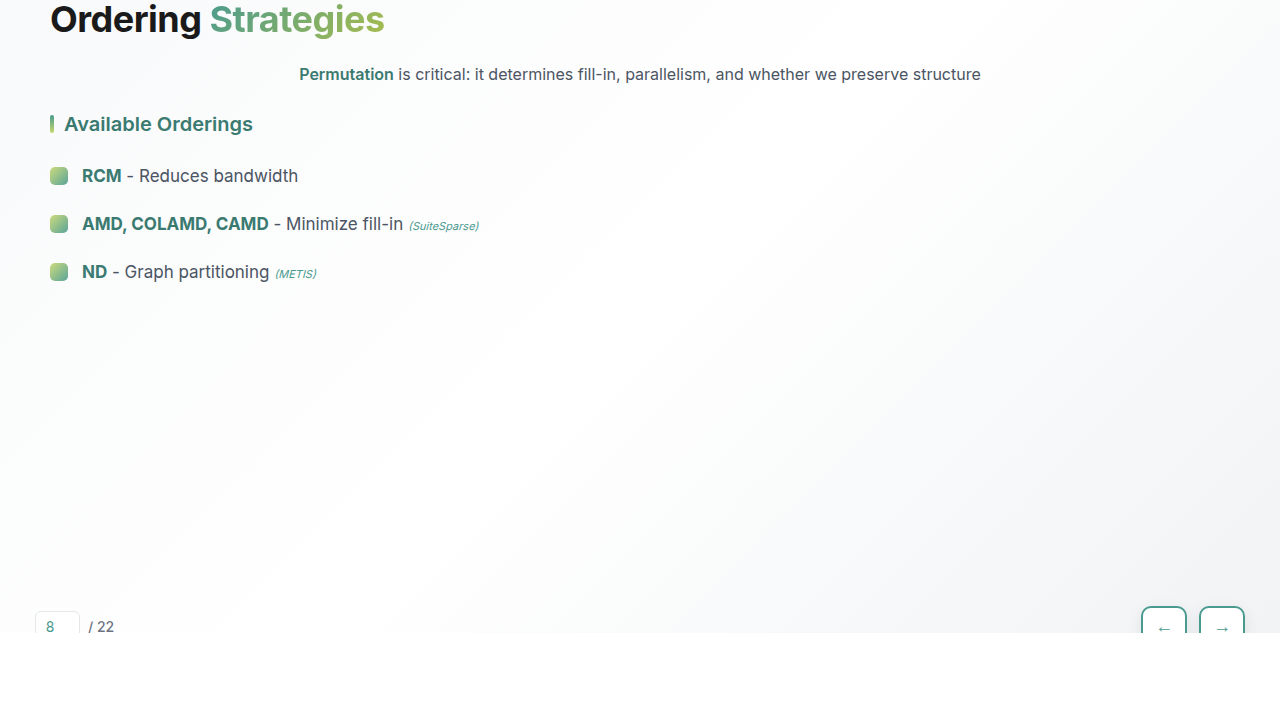
\includegraphics[width=\textwidth]{slide_screenshots/slide_08.png}
\end{center}
%==============================================================================

\begin{speech}
Permutation is critical in sparse factorization. The ordering determines fill-in, parallelism, and whether we preserve the matrix structure.

We support multiple orderings: RCM for bandwidth reduction, AMD and variants from SuiteSparse for fill-in minimization, and Nested Dissection via METIS for graph partitioning.

\textit{[Advance to show METIS limitation]}

Nested Dissection is attractive because partitions can be processed in parallel. However, METIS isn't always optimal for our matrices. It often creates imbalanced partitions with uneven task distribution, which hurts parallel efficiency.

\textit{[Advance to show our approach]}

Our approach includes adapted Nested Dissection that balances partition sizes, custom structure-aware orderings, and hybrid combinations.

We can also do tile-level ordering --- permuting the tiles themselves after the initial partitioning. And hierarchical approaches: global ND with METIS, then different local orderings per partition.
\end{speech}

\vspace{1em}

%==============================================================================
\section{Ordering Strategies (continued)}
\begin{center}
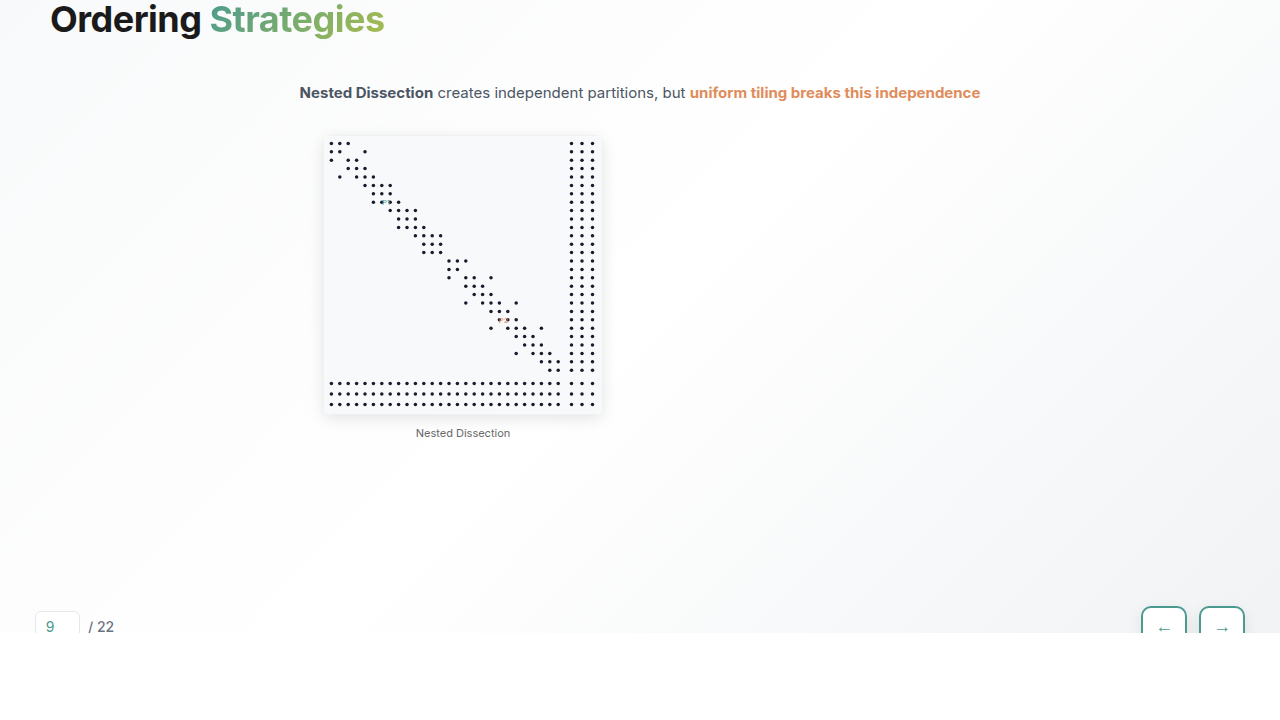
\includegraphics[width=\textwidth]{slide_screenshots/slide_09.png}
\end{center}
%==============================================================================

\begin{speech}
Here's an important subtlety: Nested Dissection creates independent partitions at the element level, but uniform tiling can break this independence.

Look at this example. The original sparse matrix after ND has independent blocks. But when we overlay a uniform tile grid, tiles can span partition boundaries. A single tile might contain elements from multiple partitions.

This introduces dependencies between what were supposed to be independent blocks. We have to account for this in our scheduling.

Our adapted ND approach adjusts the separator position to align better with tile boundaries, preserving more of the partition independence at the tile level.
\end{speech}

\vspace{1em}

%==============================================================================
\section{Tree Reduction Explained}
\begin{center}
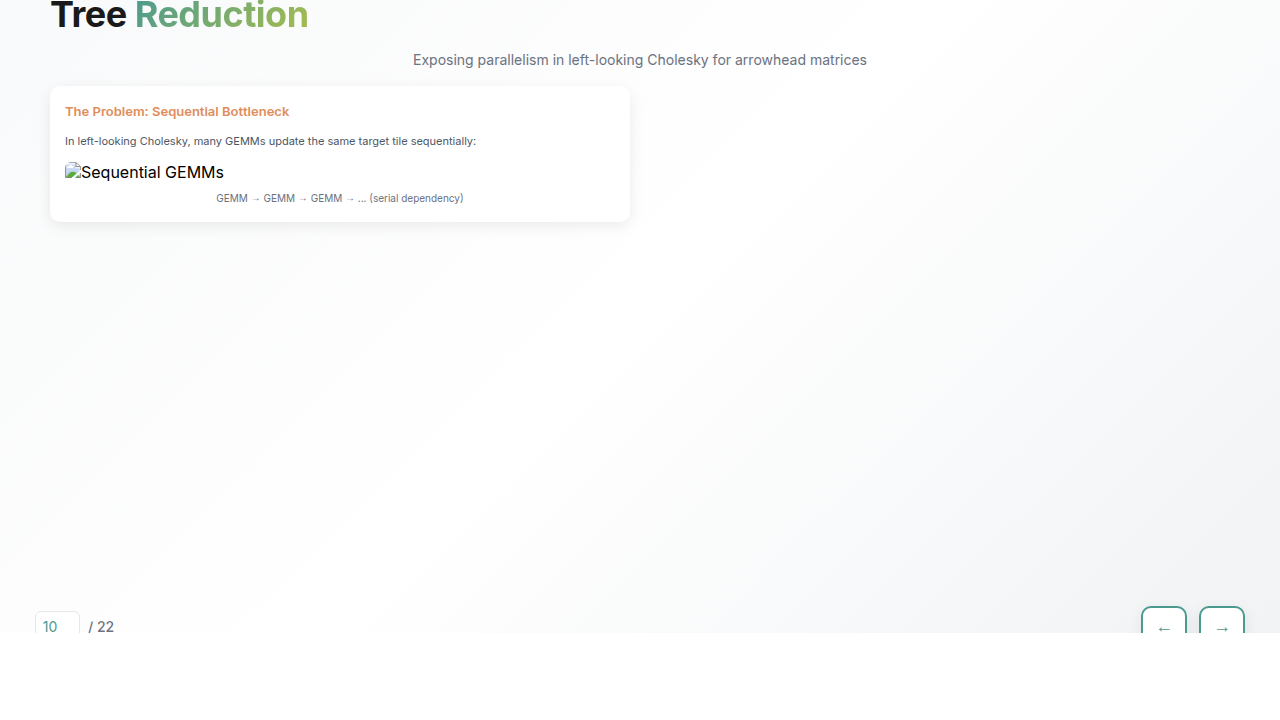
\includegraphics[width=\textwidth]{slide_screenshots/slide_10.png}
\end{center}
%==============================================================================

\begin{speech}
The arrowhead matrix structure creates a parallelism challenge. Look at the DAG for a dense matrix versus an arrowhead matrix. The dense DAG is wide, exposing massive parallelism. The arrowhead DAG is \textbf{thin} --- there's a long chain of dependent operations.

The problem is in the left-looking Cholesky variant: many GEMM operations update the same target tile sequentially. This creates a bottleneck.

Tree reduction solves this. Instead of sequential GEMMs accumulating to one tile, each core computes GEMMs to its own temporary tile in parallel. Then we use a tree-based reduction with GEADD operations to combine the results.

The reduction depth is $\log_2(n)$, so even with thousands of GEMMs, we only need a handful of reduction levels.

The condition: tree reduction helps when the number of accumulations is at least twice the number of available cores. For thick arrowhead matrices with high bandwidth, this is always satisfied.
\end{speech}

\vspace{1em}

%==============================================================================
\section{Algorithm Pipeline}
\begin{center}
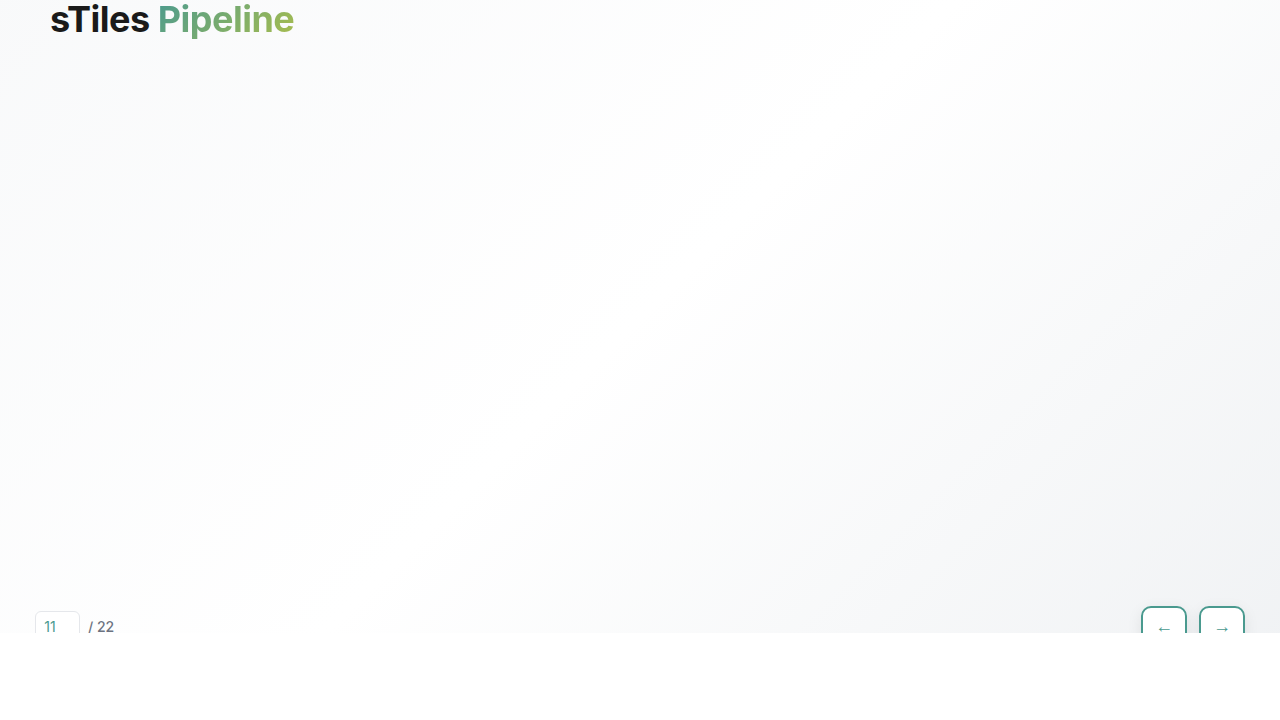
\includegraphics[width=\textwidth]{slide_screenshots/slide_11.png}
\end{center}
%==============================================================================

\begin{speech}
Let me walk through the complete sTiles pipeline.

First, preprocessing: we apply permutation --- chosen based on matrix structure --- then symbolic factorization to identify nonzero tiles. We allocate only the tiles that will be non-zero.

The numerical factorization uses a customized static scheduler. Each thread has a pre-computed Task Assignment Table --- no runtime scheduling overhead. We use a left-looking variant with tree reduction for the accumulation bottleneck.

For GPU execution, each CPU thread manages its own CUDA stream. We replace CPU kernels with cuBLAS and cuSOLVER equivalents: cusolverDnDpotrf, cublasDsyrk, cublasDtrsm, cublasDgemm.

Selected inversion follows the same tile-based approach, computing only the elements of $A^{-1}$ that correspond to the original sparsity pattern.
\end{speech}

\vspace{1em}

%==============================================================================
\section{Test Matrix Characteristics}
\begin{center}
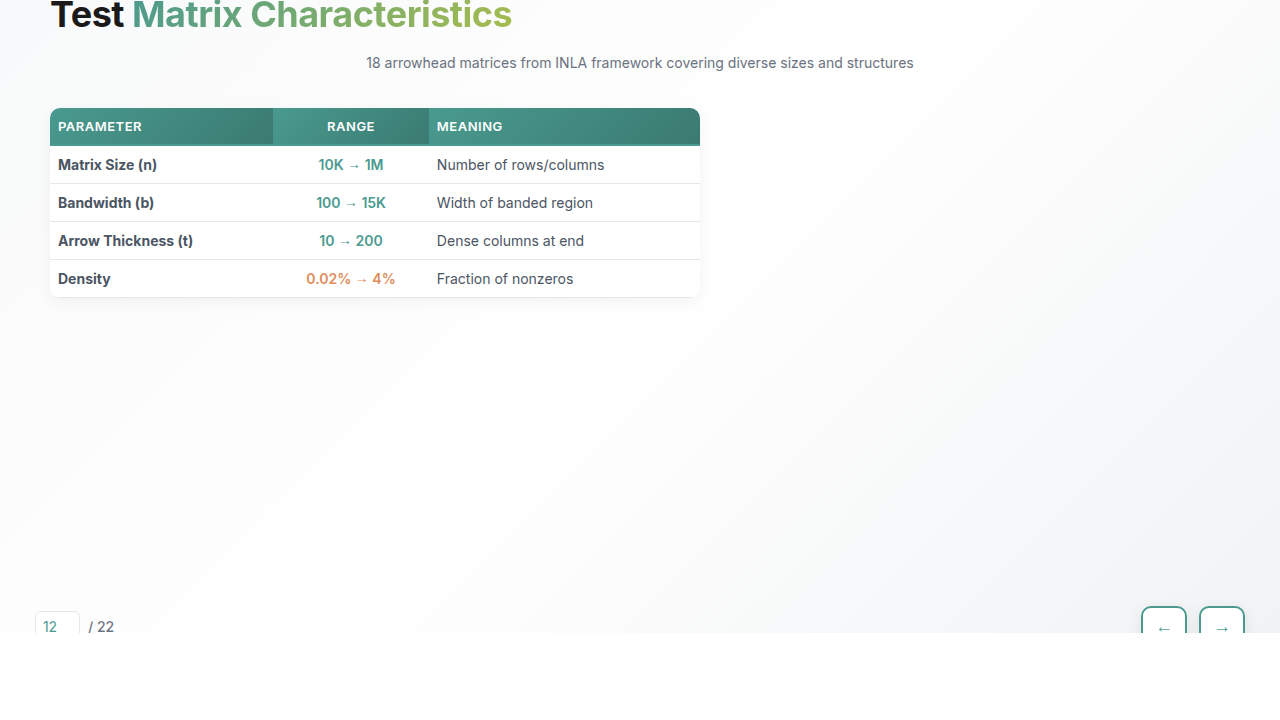
\includegraphics[width=\textwidth]{slide_screenshots/slide_12.png}
\end{center}
%==============================================================================

\begin{speech}
For our experimental evaluation, we use test matrices representative of real INLA applications.

The matrices span three size groups: 10K, 100K, and 500K rows. Within each group, we vary bandwidth from 100 to 3000, and arrowhead thickness of 10 or 200.

Matrix IDs 1 through 18 cover this parameter space. The bandwidth corresponds to the width of the banded diagonal, while arrowhead thickness represents dense blocks at the end --- typically fixed effects in statistical models.

For GPU experiments, we add larger matrices: 50K with bandwidth 15,000 to stress-test GPU kernels, and 1 million rows for scalability testing.

These matrices arise from Kronecker products of spatial and temporal precision matrices, exactly what you'd encounter in spatiotemporal statistics.
\end{speech}

\vspace{1em}

%==============================================================================
\section{Performance: Cholesky Factorization}
\begin{center}
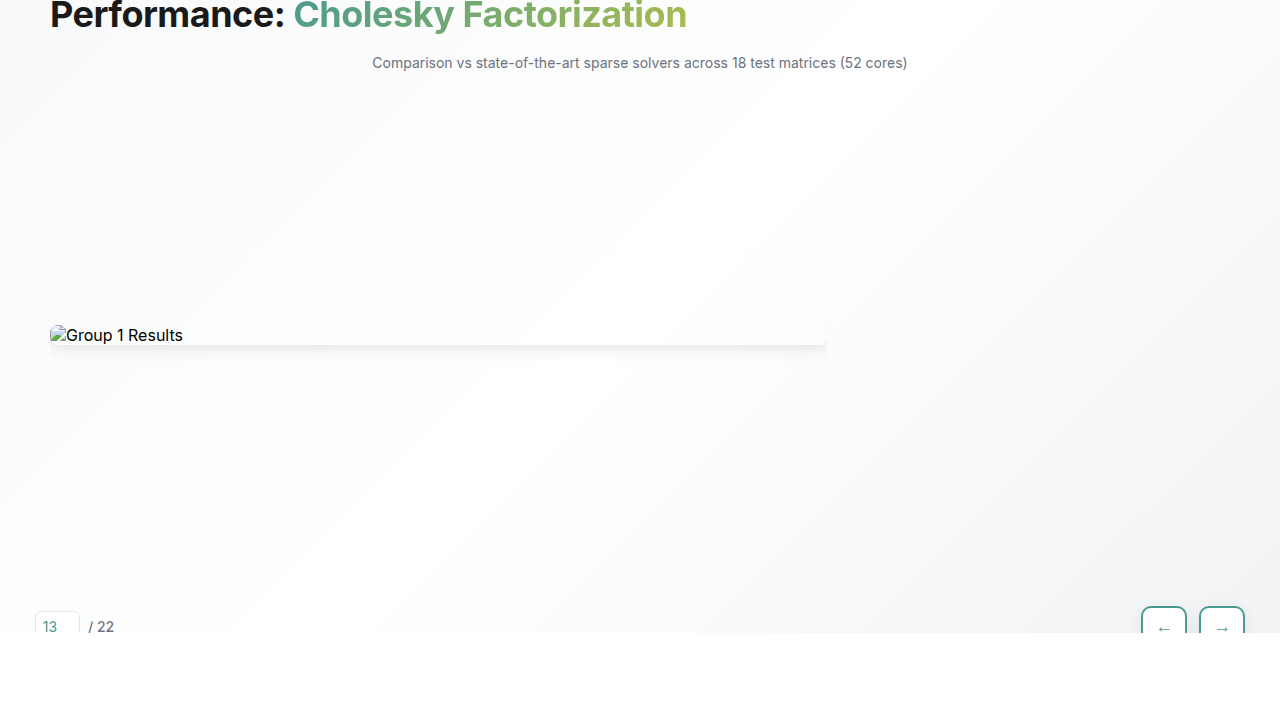
\includegraphics[width=\textwidth]{slide_screenshots/slide_13.png}
\end{center}
%==============================================================================

\begin{speech}
Now for the results. This slide compares sTiles against state-of-the-art sparse solvers: CHOLMOD, SymPACK, MUMPS, and PARDISO.

The plots show execution time for our test matrices on a 52-core Intel Xeon system. Lower is better.

\textit{[Advance to show second plot]}

For larger matrices, especially those with higher bandwidth, sTiles dominates.

\textit{[Advance to show speedup summary]}

The maximum speedups are striking: 11× over PARDISO, 9.3× over SymPACK, 8.4× over CHOLMOD, 5× over MUMPS.

Critically, the performance gap \textbf{grows with matrix size}. sTiles scales better because our tile-based approach with static scheduling eliminates the overhead that dynamic approaches accumulate at scale.
\end{speech}

\vspace{1em}

%==============================================================================
\section{Non-Arrowhead Cases: General Sparse Matrices}
%==============================================================================

\begin{speech}
sTiles is not limited to arrowhead structures. To demonstrate generality, we tested on three SuiteSparse matrices with general sparse patterns: msc23052, ship\_001, and nd6k.

\textit{[Click: msc23052 appears]}

msc23052 has 23,052 rows and 588,933 nonzeros. PARDISO is faster here --- this matrix is small and sparse, where its supernodal approach has an advantage. sTiles best time is 0.077s at 32 threads.

\textit{[Click: ship\_001 appears]}

ship\_001 has 34,920 rows and nearly 4 million nonzeros. A denser matrix. Both solvers reach around 64--74 milliseconds at 32 threads --- very close performance.

\textit{[Click: nd6k appears]}

nd6k is the most demanding: 18,000 rows but 6.9 million nonzeros --- very dense for its size. Here sTiles wins: 0.351s at 16 threads versus PARDISO's best of 0.483s at 32 threads. High density plays to sTiles' strength: dense tiles enable efficient BLAS kernels.

The takeaway: on denser general sparse matrices, sTiles wins. Even on smaller sparser cases where PARDISO excels, sTiles remains competitive.
\end{speech}

\vspace{1em}

%==============================================================================
\section{Performance: Tree Reduction}
\begin{center}
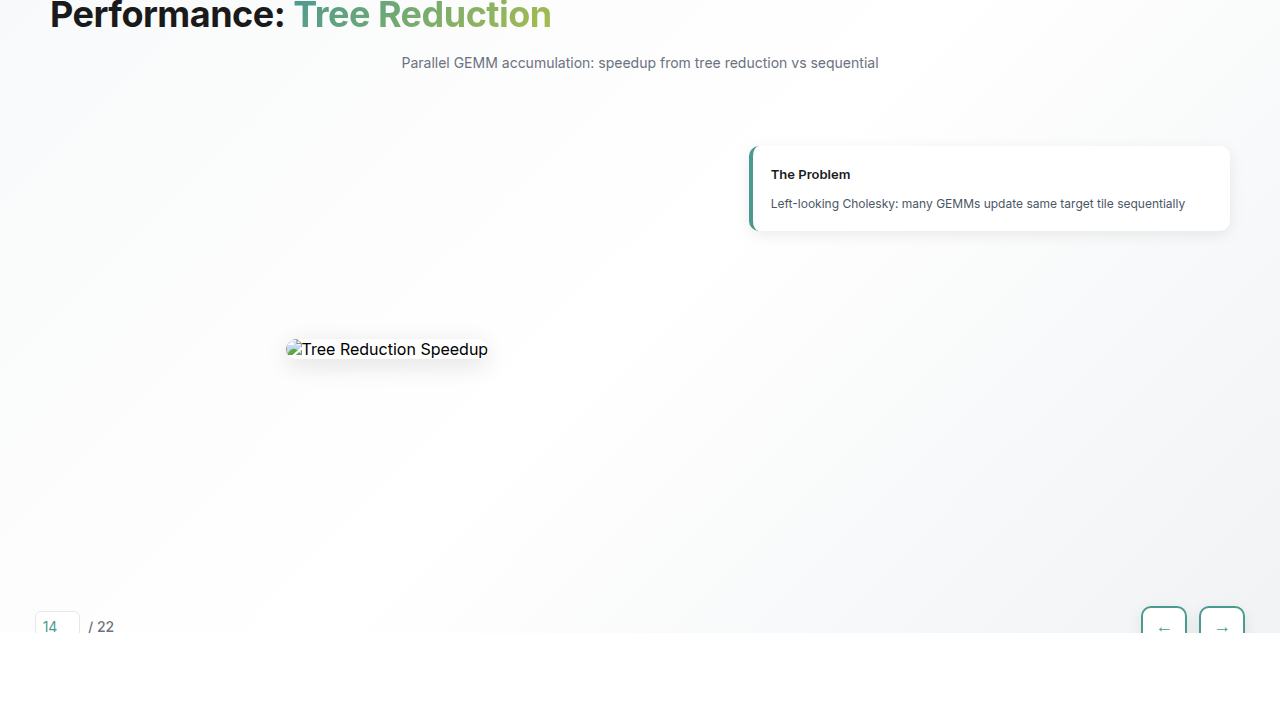
\includegraphics[width=\textwidth]{slide_screenshots/slide_14.png}
\end{center}
%==============================================================================

\begin{speech}
This plot shows the benefit of tree reduction for parallel GEMM accumulation.

The x-axis is core count, y-axis is speedup versus sequential execution. Different curves represent different numbers of GEMMs to accumulate.

For 50,000 GEMMs, tree reduction achieves up to 5× speedup at 16-32 cores.

\textit{[Advance to show explanation]}

The problem: left-looking Cholesky has many GEMMs updating the same tile sequentially.

The solution: parallel GEMMs to temporary tiles, then tree-based GEADD accumulation.

The sweet spot is when you have enough GEMMs to keep all cores busy during the parallel phase, but not so many that the reduction overhead dominates.
\end{speech}

\vspace{1em}

%==============================================================================
\section{Performance: Core Scaling}
\begin{center}
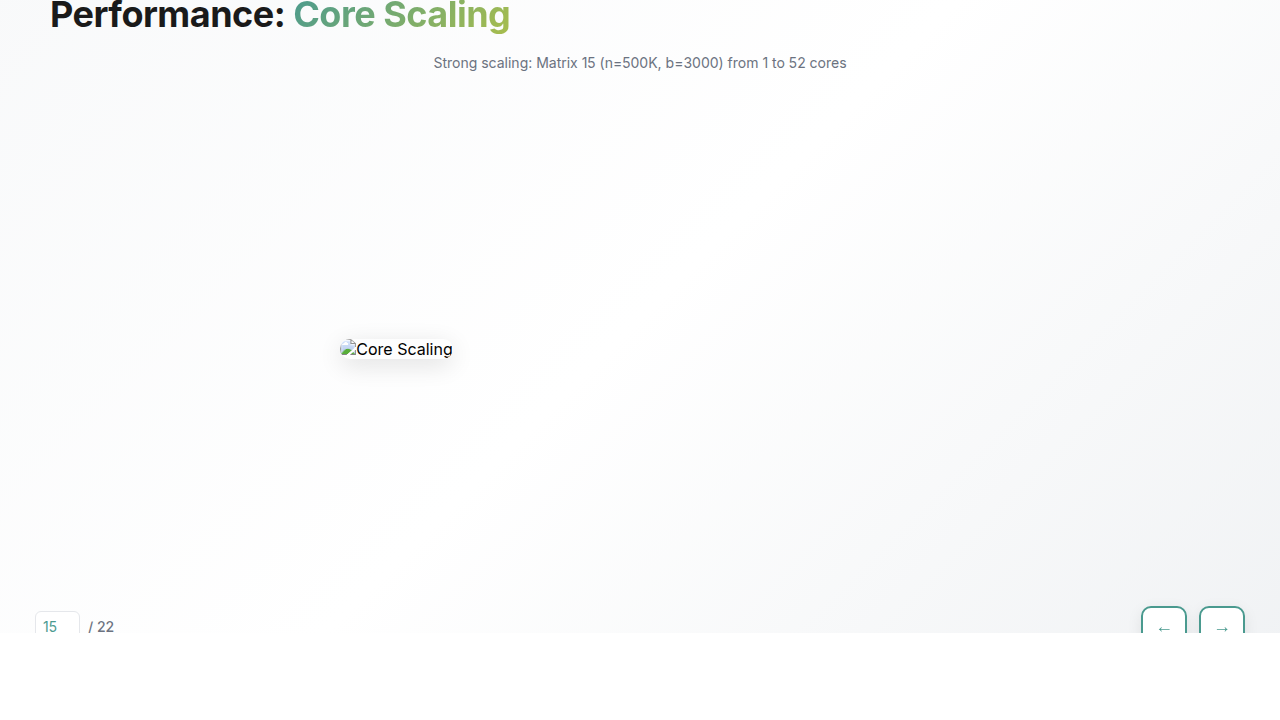
\includegraphics[width=\textwidth]{slide_screenshots/slide_15.png}
\end{center}
%==============================================================================

\begin{speech}
This is strong scaling: how execution time decreases as we add cores, for a fixed-size matrix.

We use Matrix 15 --- 500K rows, bandwidth 3000 --- scaling from 1 to 52 cores.

sTiles, shown in lime green, is fastest at all core counts. At 52 cores, it achieves 0.8 seconds versus 12.6 seconds single-threaded --- that's 15.6× speedup.

\textit{[Advance to show comparisons]}

The sparse solvers --- CHOLMOD, SymPACK, MUMPS, PARDISO --- are 3.8× to 10.7× slower than sTiles at 52 cores.

PLASMA, the dashed line, is the dense baseline. It's 271× slower because it treats the full matrix without exploiting sparsity.

\textit{[Advance to show key message]}

sTiles exploits structure: sparse storage footprint with dense BLAS kernel performance. Best of both worlds.
\end{speech}

\vspace{1em}

%==============================================================================
\section{Selected Inversion: Library Landscape}
%==============================================================================

\begin{speech}
Before showing our selected inversion results, let me explain why we benchmark against PARDISO specifically.

\textit{[Click: matrix visualization appears]}

The goal of selected inversion is to compute $A^{-1}_{ij}$ for \textit{all} $(i,j)$ in the sparsity pattern of $A$ --- not just a few entries. This is a much harder problem than computing individual elements.

\textit{[Click: MUMPS appears]}

MUMPS computes arbitrary entries of $A^{-1}$ by solving $A \cdot x = e_i$ per index via elimination tree pruning. Efficient for a handful of entries, but impractical when you need the full sparsity pattern --- thousands of solves.

\textit{[Click: PSelInv appears]}

PSelInv implements supernodal left-looking selected inversion, used in the PEXSI library. On our large structured problems it is slower than PARDISO and ran out of memory in several cases. Additionally, PEXSI is no longer actively maintained.

\textit{[Click: Serinv appears]}

Serinv is a recent specialized library, but restricted to block-tridiagonal + arrowhead matrices only. sTiles targets \textit{general sparse SPD} matrices beyond this fixed structure.

\textit{[Click: PARDISO appears]}

PARDISO implements state-of-the-art supernodal $LL^T$ factorization with a full selected inversion routine. It is the strongest available competitor for full-pattern selected inversion on structured problems --- which is why we use it as our benchmark.
\end{speech}

\vspace{1em}

%==============================================================================
\section{Performance: Selected Inversion}
\begin{center}
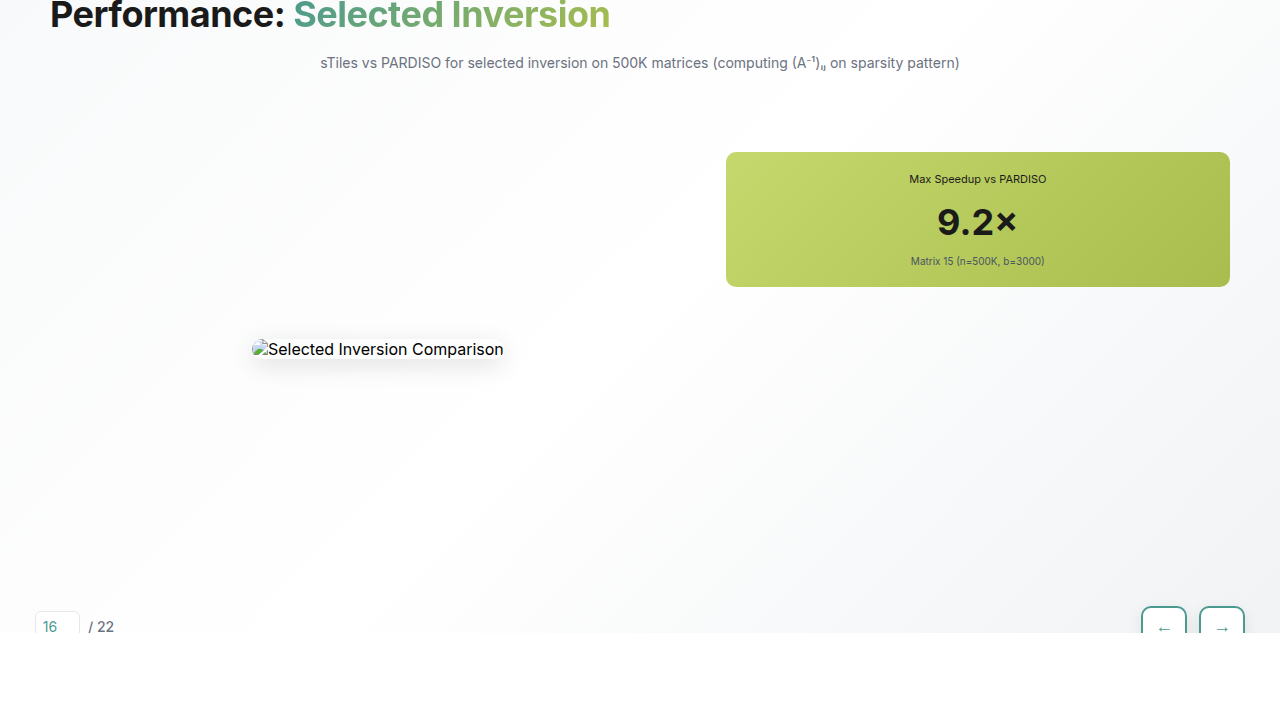
\includegraphics[width=\textwidth]{slide_screenshots/slide_16.png}
\end{center}
%==============================================================================

\begin{speech}
Now let's look at selected inversion --- computing elements of $A^{-1}$ on the sparsity pattern.

This operation is essential for Bayesian inference: we need diagonal elements for marginal variances, off-diagonals for covariances.

This plot compares sTiles versus PARDISO for selected inversion on 500K matrices.

sTiles achieves up to \textbf{9.2× speedup} over PARDISO for high-bandwidth matrices.

\textit{[Advance to show details]}

For matrices 14, 15, 17, 18 with higher bandwidth, sTiles is 2.6× to 9.2× faster.

For low-bandwidth matrices like 13 and 16, performance is similar --- sparse overhead dominates when there's not enough computational work per tile.

The key insight: our tile-based approach with static scheduling eliminates dynamic overhead that becomes significant at scale.
\end{speech}

\vspace{1em}

%==============================================================================
\section{Selected Inversion: Density Effect}
\begin{center}
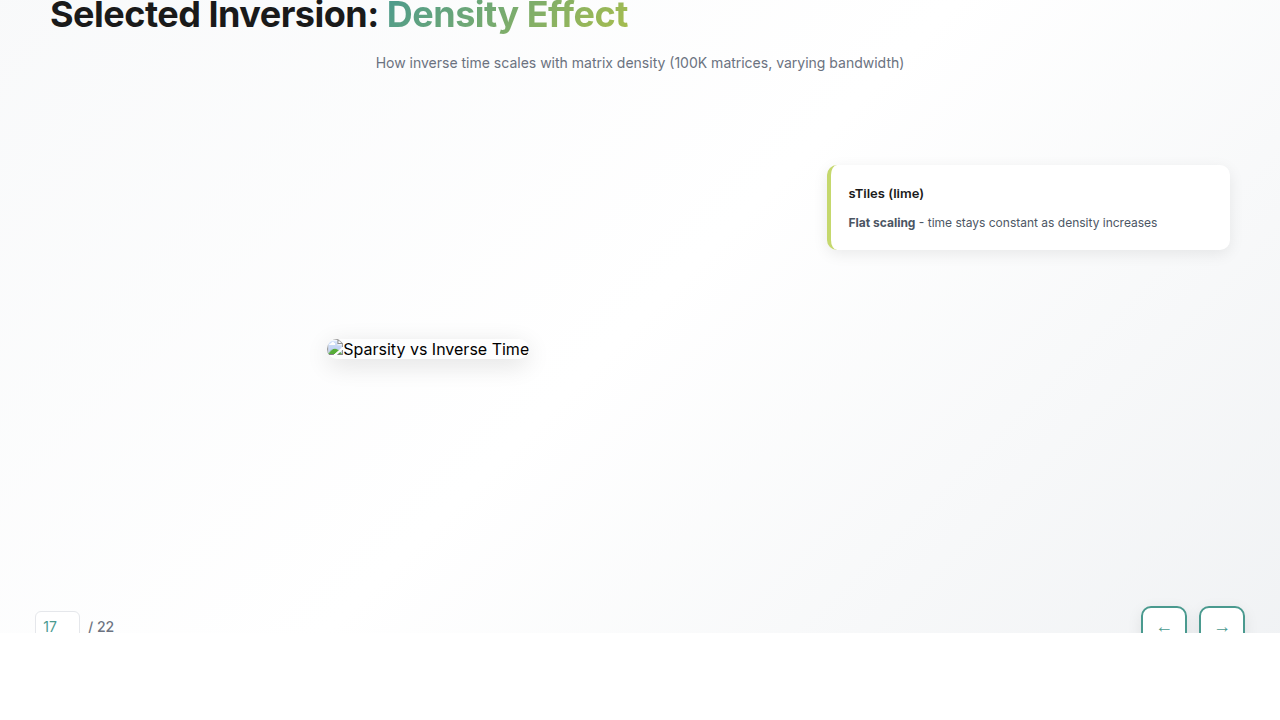
\includegraphics[width=\textwidth]{slide_screenshots/slide_17.png}
\end{center}
%==============================================================================

\begin{speech}
This experiment examines how selected inversion time scales with matrix density.

We use 100K matrices with increasing density. Two sets: Set~1 with bandwidth 1500, Set~2 with bandwidth 3000.

The speedup range of sTiles over PARDISO spans 0.15$\times$ to 12$\times$ for Set~1, and 0.09$\times$ to 7.4$\times$ for Set~2. The lower bound --- below 1$\times$ --- occurs at very low density where PARDISO's supernodal approach has an advantage and sTiles carries some tile overhead.

sTiles, shown in lime, has \textbf{remarkably flat scaling}. Execution time stays nearly constant as density increases.

\textit{[Advance to show PARDISO]}

PARDISO, in black, shows growing cost --- time increases significantly with density. At high density, sTiles reaches up to 12$\times$ speedup for Set~1 and 7.4$\times$ for Set~2.

\textit{[Advance to show explanation]}

Why does sTiles stay flat? Fixed tile size means predictable BLAS workload. Once a tile is allocated, we process it the same way regardless of how many nonzeros are inside.

PARDISO's supernodal approach is more sensitive to actual fill within supernodes --- denser matrices mean larger supernodes and more fill-in overhead.
\end{speech}

\vspace{1em}

%==============================================================================
\section{GPU Acceleration}
\begin{center}
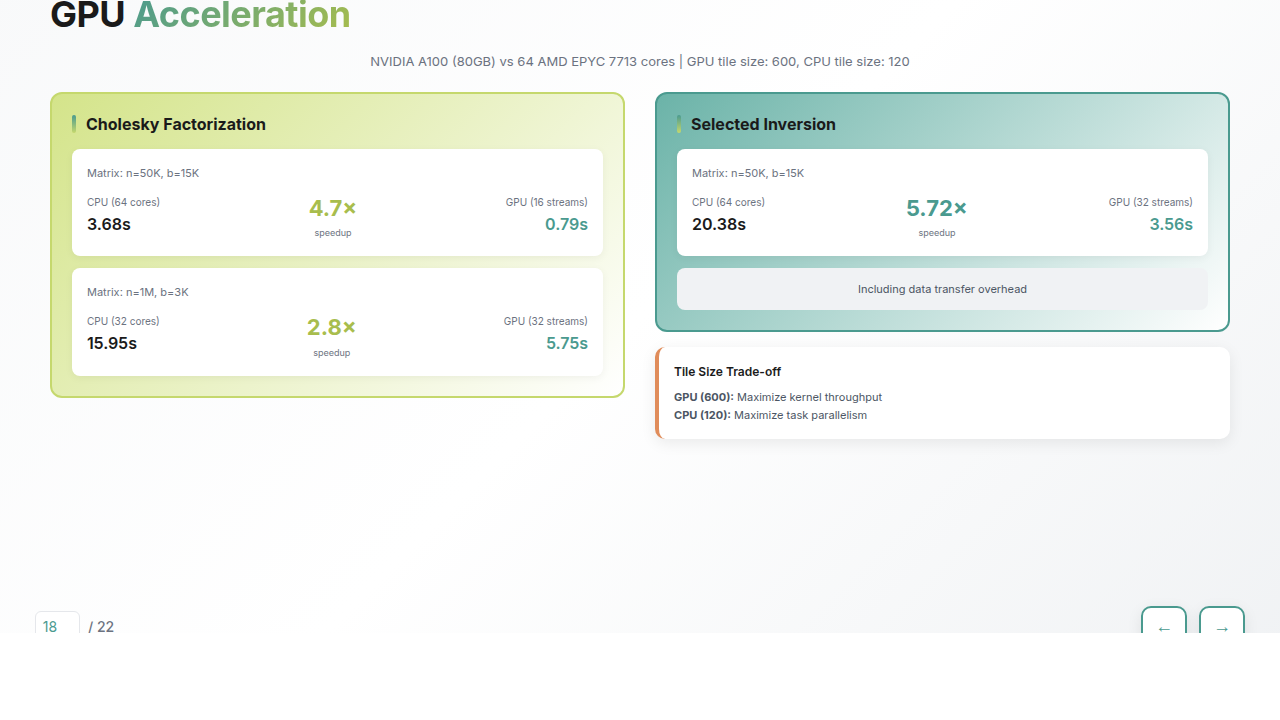
\includegraphics[width=\textwidth]{slide_screenshots/slide_18.png}
\end{center}
%==============================================================================

\begin{speech}
Finally, GPU acceleration. We compare an NVIDIA A100 with 80GB memory against a 64-core AMD EPYC CPU.

For Cholesky factorization: the 50K matrix with bandwidth 15K achieves 4.7× GPU speedup --- 0.79 seconds on GPU versus 3.68 seconds on 64 CPU cores.

The larger 1M matrix with bandwidth 3K achieves 2.8× speedup. Lower relative speedup because the narrower bandwidth means less computational intensity per tile.

For selected inversion: the 50K matrix achieves 5.7× GPU speedup. Selected inversion has more computation per memory access than factorization, making it even more GPU-friendly.

The GPU implementation uses larger tiles --- 600 instead of 120 --- to maximize kernel efficiency. Each CPU thread manages its own CUDA stream for concurrent kernel execution.
\end{speech}

\vspace{1em}

%==============================================================================
\section{Dense Matrix Performance}
\begin{center}
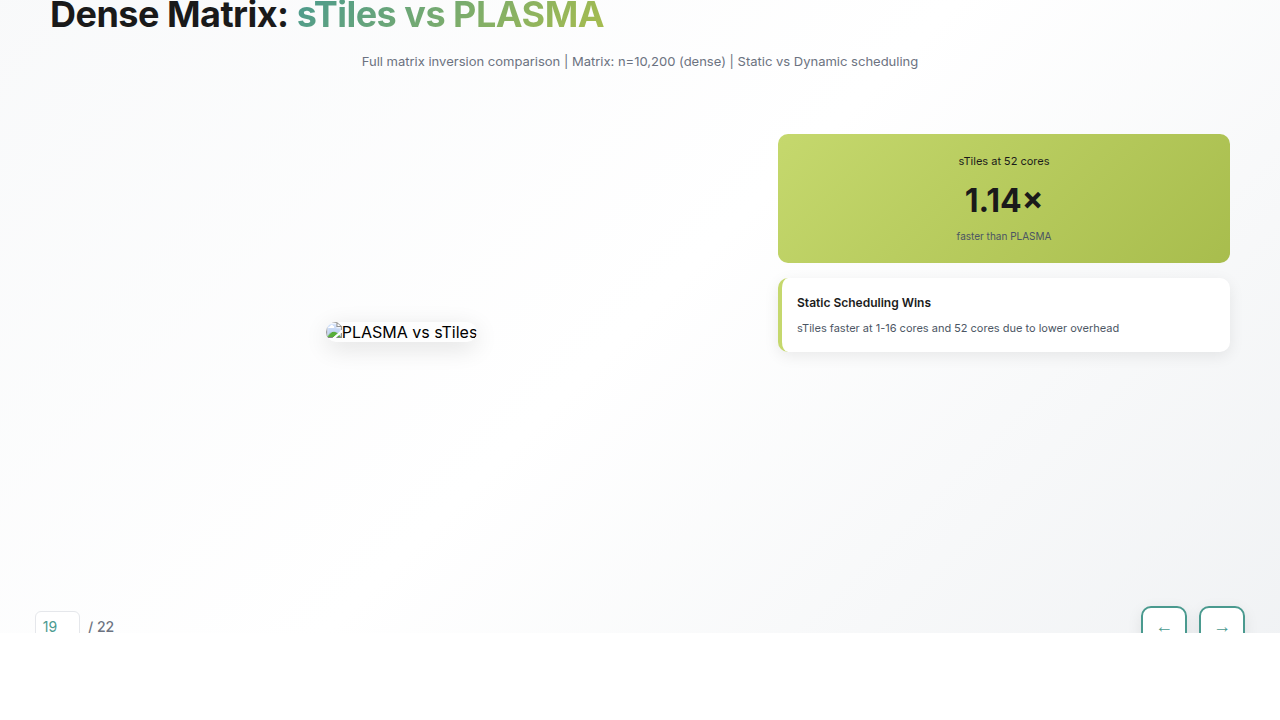
\includegraphics[width=\textwidth]{slide_screenshots/slide_19.png}
\end{center}
%==============================================================================

\begin{speech}
For completeness, we also show sTiles performance on fully dense matrices --- the limiting case where every tile is nonzero.

Even here, sTiles is competitive with PLASMA, the state-of-the-art dense solver. Both use the same underlying BLAS kernels; sTiles adds minimal overhead from its sparse-aware infrastructure.

This validates that sTiles doesn't sacrifice dense performance to gain sparse efficiency. When the matrix happens to be dense, we match the dense solver performance. When it's sparse, we dramatically outperform sparse solvers.
\end{speech}

\vspace{1em}

%==============================================================================
\section{Key Innovations}
%==============================================================================

\begin{speech}
Let me summarize the key innovations in sTiles.

First, \textbf{tile-based hybrid approach}: uniform tiles with dense BLAS kernels, but operating only on nonzero tiles. This bridges sparse and dense linear algebra.

Second, \textbf{structure-aware scheduling}: static task assignment eliminates runtime overhead. Each core knows exactly what to compute before numerical work begins.

Third, \textbf{tree reduction}: breaks the sequential bottleneck in left-looking Cholesky for arrowhead matrices.

Fourth, \textbf{GPU acceleration}: larger tiles for GPU efficiency, CUDA streams for concurrency, cuBLAS/cuSOLVER kernels.

Fifth, \textbf{flexible ordering}: supports RCM, AMD, ND, and hybrid combinations, with automatic selection based on matrix structure.

These innovations combine to deliver order-of-magnitude speedups over existing solvers for structured sparse matrices.
\end{speech}

\vspace{1em}

%==============================================================================
\section{Publications and Future Work}
\begin{center}

\includegraphics[width=\textwidth]{slide_screenshots/slide_20.png}
\end{center}
%==============================================================================

\begin{speech}
This work is documented in two papers.

The first, on Cholesky factorization, was published at ISC High Performance 2025. It covers the sTiles framework, tile algorithms, ordering strategies, tree reduction, and CPU/GPU performance.

The second, on selected inversion, is targeting ISC 2026. It extends sTiles to compute inverse elements on the sparsity pattern, with the two-phase algorithm and additional GPU optimizations.

For future work, we're exploring multi-GPU support for even larger matrices, distributed memory implementations for cluster-scale problems, and integration with R-INLA for direct impact on statistical applications.

The software is open source, available on GitHub.
\end{speech}

\vspace{1em}

%==============================================================================
\section{Summary}
\begin{center}
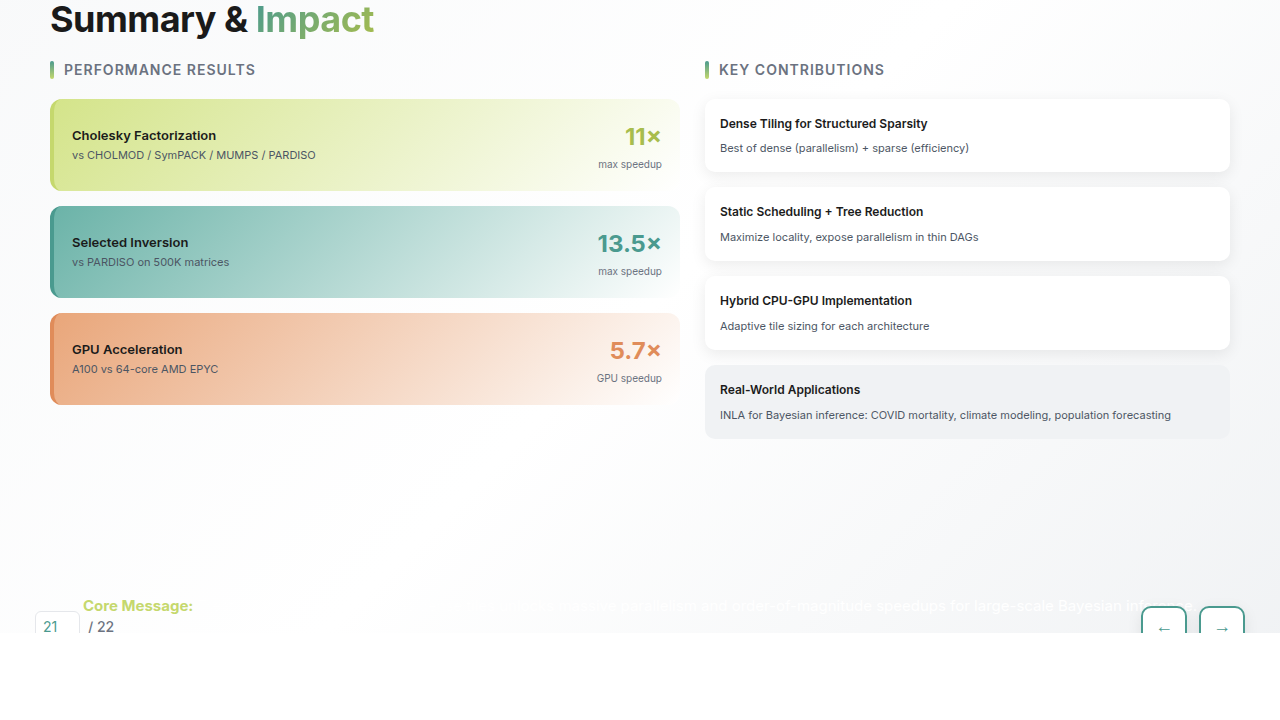
\includegraphics[width=\textwidth]{slide_screenshots/slide_21.png}
\end{center}
%==============================================================================

\begin{speech}
To summarize:

sTiles is a GPU-accelerated framework for sparse factorizations of structured matrices, particularly arrowhead patterns from Bayesian inference.

The key insight: combine sparse techniques --- permutation, symbolic factorization, skipping zeros --- with dense performance from tile-based BLAS-3 operations.

Results for Cholesky factorization: up to 11× speedup over PARDISO, with the gap growing at larger scales.

Results for selected inversion: up to 9.2× speedup over PARDISO on CPU, additional 5.7× speedup on GPU.

The practical impact: enabling faster Bayesian inference for large-scale spatial and spatiotemporal statistics, where these factorizations are often the computational bottleneck.
\end{speech}

\vspace{1em}

%==============================================================================
\section{Thank You}
\begin{center}
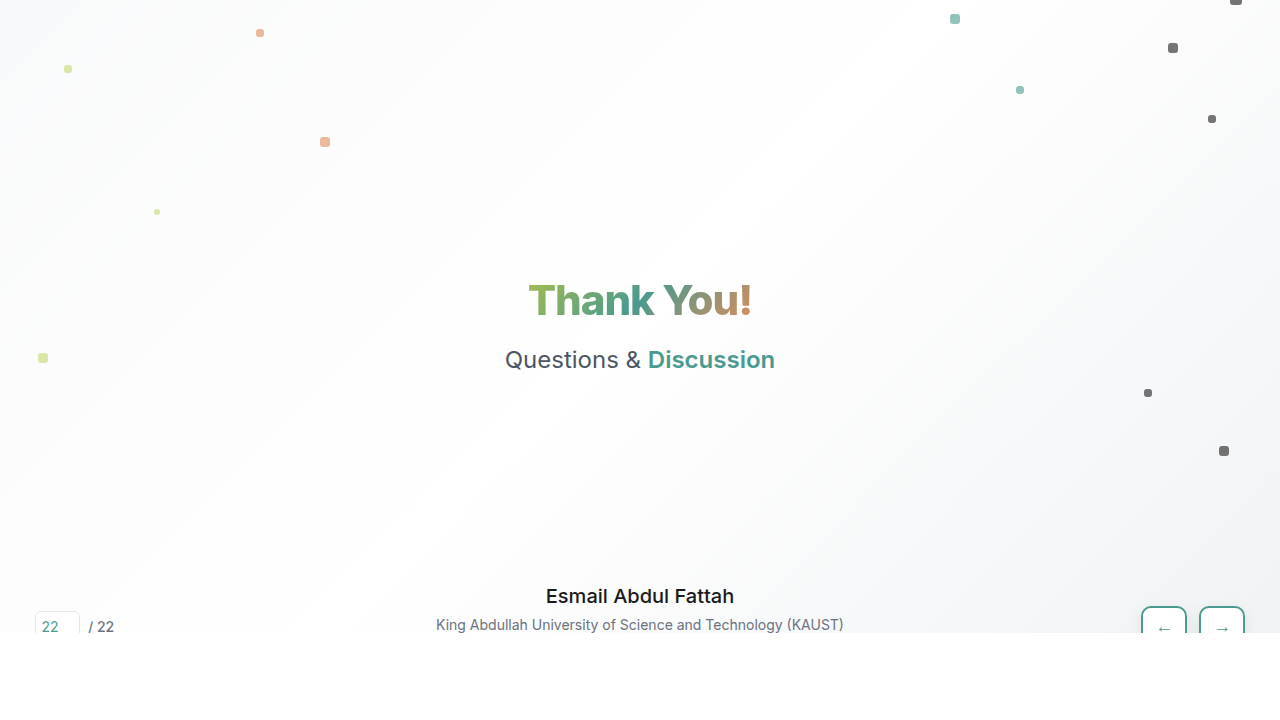
\includegraphics[width=\textwidth]{slide_screenshots/slide_22.png}
\end{center}
%==============================================================================

\begin{speech}
Thank you for your attention.

The sTiles software is available at github.com/esmail-abdulfattah/sTiles.

I'm happy to take questions about the algorithms, implementation details, or results.
\end{speech}

\vspace{2em}
\hrule
\vspace{1em}

\begin{center}
\textit{End of presentation script}
\end{center}

\end{document}
